% ICASSP 2027 submission (single-blind). Built with spconf.sty and IEEEbib.bst; compile with `make paper`.
% Every number in this file comes from a committed report in outputs/reports/ (cited per table in comments).
\documentclass{article}
\usepackage{spconf,amsmath,graphicx,booktabs,multirow,array}
\usepackage[hyphens]{url}
\usepackage[hidelinks]{hyperref}
\usepackage{enumitem,xcolor}
\graphicspath{{../outputs/figures/}}
\setlist{nosep,leftmargin=*}

\emergencystretch=1em  % avoids overfull lines in the narrow columns
\newcommand{\gpt}{GPT-Audio-1.5}
\newcommand{\gem}{Gemini 3.8 Flash}
\newcommand{\qwen}{Qwen2.5-Omni-7B}
\newcommand{\af}{Audio Flamingo 3}

\title{Reference Agreement Is Not Acoustic Correctness: Evaluating Large Audio Language Model Captions Against Human References on Clotho}

\name{Anandaswarup Vadapalli}
\address{International Institute of Information Technology, Hyderabad, India}

\begin{document}
\ninept
\maketitle

\begin{abstract}
Large audio language models (LALMs) describe sound recordings fluently, but their captions
are usually judged by how closely they agree with human references. We evaluate captions from four LALMs, \gpt, \gem,
\qwen\ and \af, on the complete Clotho v2.1 evaluation split (1,045 recordings, 5,225 human captions) with twelve
reference-based and two audio-aware metrics. A matched leave-one-out procedure scores held-out human captions against
the same four references as the models. The two open-weight models score highest on every reference-based metric,
yet all four models remain below the human baseline on each of them; only \af\ on CLAP audio--text similarity is not
significantly different from it. Model captions are 1.4--1.9 times longer than human captions, and longer captions
score lower on overlap metrics. A single-reviewer audit of 200 sampled captions against the audio reverses the model
order: \gpt, ranked third or fourth by the text metrics, was rated accurate for 47 of 50 recordings, and 56 of the 64
captions that disagree most with the references had no major error. No evaluated metric showed significantly
above-chance within-recording concordance with the audio ratings in this sample. Reference agreement alone is
therefore insufficient evidence of acoustic correctness.
\end{abstract}

\begin{keywords}
Audio captioning, large audio language models, evaluation metrics, Clotho, human references
\end{keywords}

\section{Introduction}
\label{sec:intro}

Automated audio captioning (AAC) describes the sound sources, events and acoustic characteristics of a recording in
natural language~\cite{mei2022overview}. Applications include accessibility, multimedia retrieval and soundscape
analysis. Large audio language models (LALMs) now perform this task without task-specific training, and produce
longer and more detailed descriptions than captioning systems trained on AAC
datasets~\cite{gong2024ltu,tang2024salmonn,xu2025qwen25omni,ghosh2025af3}.

AAC systems are evaluated by comparing their captions with human references. Metrics such as BLEU~\cite{papineni2002bleu},
METEOR~\cite{banerjee2005meteor}, CIDEr~\cite{vedantam2015cider} and SPIDEr~\cite{liu2017spider} measure the lexical
or semantic overlap between a caption and the references. A recording, however, often contains several sounds, and
different listeners describe different aspects of it. A caption may therefore describe an audible event that no
reference mentions and receive a low score, or overlap well with the references while misrepresenting the audio. The
difference matters more for LALMs, whose captions differ from the references in length and style.

In this paper we compare captions from four LALMs with the human references of Clotho v2.1~\cite{drossos2020clotho}.
We address three research questions:

\begin{enumerate}
\item \textbf{RQ1: How closely do model captions agree with the five human reference captions?} We score each
model's caption against all five references of its recording with twelve reference-based metrics and two
audio-aware metrics, and compare the models.
\item \textbf{RQ2: How do model captions compare with held-out human captions in metric scores and caption length?}
We score each human caption against the other four references and each model caption against the same four, so that
model and human scores are directly comparable. We also compare caption lengths.
\item \textbf{RQ3: What patterns of agreement, additional detail, omission and mismatch appear in model captions?}
We review a random sample of 200 model captions first against the references and then against the audio, and test
whether the metrics follow either review.
\end{enumerate}

We find that the reference-based metrics agree with each other and with the reference-only review, but we find no
evidence that they follow correctness against the audio. The model with the most accurate captions in the audio review ranks third or fourth on
every text metric. Section~\ref{sec:related} reviews related work, Section~\ref{sec:method} describes the methodology,
Section~\ref{sec:results} presents the results for RQ1--RQ3, Section~\ref{sec:discussion} discusses their
implications, and Section~\ref{sec:limitations} states the limitations.

\section{Related Work}
\label{sec:related}

\subsection{Automated audio captioning}
\label{ssec:rw-aac}

AAC research relies on two crowdsourced datasets, AudioCaps~\cite{kim2019audiocaps} and
Clotho~\cite{drossos2020clotho}, and has been driven by the DCASE challenge since 2020~\cite{mei2022overview}.
AudioCaps provides one caption per training recording and five per test recording, drawn from AudioSet. Clotho provides
five captions for each of its 15--30\,s recordings, collected with a three-step protocol in which annotators write
captions, other annotators correct or rephrase them, and the five captions rated highest for accuracy and fluency are
kept~\cite{lipping2019crowdsourcing}. Because both datasets are small, recent systems are pre-trained on larger,
weakly labelled caption collections such as WavCaps~\cite{mei2024wavcaps}. Human references are therefore short, single
sentences that describe the most salient sounds, and the style of these references shapes both training and evaluation.

\subsection{Large audio language models}
\label{ssec:rw-lalm}

LALMs couple a pre-trained audio encoder with a large language model and are trained to follow free-form instructions
about audio. Pengi~\cite{deshmukh2023pengi} framed audio tasks as text generation, LTU~\cite{gong2024ltu} and
SALMONN~\cite{tang2024salmonn} added open-ended question answering and reasoning, and Qwen-Audio~\cite{chu2023qwenaudio}
scaled multi-task pre-training across speech, sound and music. Recent models handle audio within general multimodal
assistants, such as Qwen2.5-Omni~\cite{xu2025qwen25omni}, or are trained specifically for audio understanding and
reasoning, such as Audio Flamingo 3~\cite{ghosh2025af3}. These models are usually evaluated on captioning benchmarks
with the same reference-based metrics as task-specific systems, although their captions are longer and more detailed
than the references. LALMs can also describe sounds that are not present in the recording~\cite{kuan2024hallucination},
which reference-based scores alone cannot reveal.

\subsection{Audio caption evaluation metrics}
\label{ssec:rw-metrics}

Most AAC metrics were borrowed from image captioning and machine translation: BLEU~\cite{papineni2002bleu},
METEOR~\cite{banerjee2005meteor} and CIDEr~\cite{vedantam2015cider} measure $n$-gram overlap, SPICE~\cite{anderson2016spice}
compares scene graphs parsed from the captions, and SPIDEr~\cite{liu2017spider} averages CIDEr and SPICE. Zhou et
al.~\cite{zhou2022fense} showed that these metrics agree poorly with human judgements of audio captions and proposed
FENSE, which combines Sentence-BERT similarity with a penalty for fluency errors. Other work scores several candidate
captions jointly~\cite{labbe2022spidermax}, measures semantic agreement of sound descriptors~\cite{wijngaard2023aces},
compares contextual token embeddings with BERTScore~\cite{zhang2020bertscore}, or asks a large language model to judge
captions~\cite{wu2025claira}. All of these metrics compare a caption with human references. Audio-aware metrics use
the recording instead: CLAP~\cite{elizalde2023clap,elizalde2024msclap} embeds audio and text in a joint space, so a
caption can be scored against the audio, as CLIPScore~\cite{hessel2021clipscore} does for images, and
MACE~\cite{dixit2025mace} combines CLAP audio--text and text--text similarity with a fluency penalty.

\subsection{Reference agreement and acoustic grounding}
\label{ssec:rw-grounding}

Scores against human references are hard to interpret without knowing how well humans agree with each other. In image
captioning, human captions scored against the remaining references give such a reference point~\cite{chen2015coco},
and object hallucination is measured by checking caption content against the image rather than against the
references~\cite{rohrbach2018chair}. Studies of AAC metrics have compared metric scores with human preferences
between caption pairs, judged on description accuracy and fluency~\cite{zhou2022fense,dixit2025mace}; they do not
rate each caption against a correctness rubric or check the details that no reference supports. This work combines
both ideas for LALM audio captions: we calibrate model scores with a matched human leave-one-out
baseline, and we verify each sampled caption, and each detail that no reference supports, against the audio.

\section{Methodology}
\label{sec:method}

\subsection{Data and models}
\label{ssec:data}

We use the complete evaluation split of Clotho v2.1~\cite{drossos2020clotho}: 1,045 recordings of 15--30\,s
(6.5\,h in total), each with five human captions of 8--20 words (5,225 captions). We evaluate two API models, \gpt\
(\texttt{gpt-audio-1.5}) and \gem\ (\texttt{gemini-3.8-flash}), and two open-weight models, \qwen~\cite{xu2025qwen25omni}
and \af~\cite{ghosh2025af3}, at pinned checkpoint revisions. Every model received a single user turn with the full recording followed by the same
instruction, shown in the prompt template below. No references were shown, no length was imposed, and no
model-specific prompt tuning was done; only the provider-specific encoding of the audio differed.

\smallskip
\noindent\fcolorbox{black!40}{black!4}{\begin{minipage}{\dimexpr\linewidth-2\fboxsep-2\fboxrule\relax}
\small
\textbf{Prompt template} (one user turn, identical for all models)\\[2pt]
\texttt{[audio]} \emph{full recording, 15--30\,s, no cropping}\\
\texttt{[text]}\hspace{0.45em}Describe the sounds heard in this audio recording in one clear sentence that mentions the
main sound sources, audible events, and distinguishing acoustic characteristics. Do not speculate about sources or
events that are not supported by the audio. Respond with the sentence only, as plain text, without JSON, lists,
labels or other formatting.
\end{minipage}}
\smallskip

Decoding used temperature 0, top-$p$ 1 and a seed of 42 where supported; \gem\ ran at its lowest thinking level (\texttt{low}), as
thinking cannot be disabled. This gave one caption per model and recording (4,180 in total). \gpt\ sometimes answered
in JSON despite the instruction: 85 captions were plain sentences wrapped in braces and were unwrapped, and 21
malformed captions were scored as returned. Excluding the 21 affected recordings changes no model order and no
significance decision. The API models are not deterministic at temperature 0, so all results are conditional on the
released captions. Checkpoint hashes, API run dates and library versions are listed in the repository.

\subsection{Metrics and human leave-one-out calibration}
\label{ssec:metrics}

The reference-based metrics are BLEU-1 to BLEU-4, METEOR, CIDEr-D, SPICE~\cite{anderson2016spice}, SPIDEr,
SPIDEr-FL, FENSE, and the raw and baseline-rescaled F1 of BERTScore, computed on PTB-tokenized text with the aac-metrics
package~\cite{labbe2025aacmetrics}. The audio-aware metrics are CLAP similarity, the cosine between the audio and caption
embeddings of MS-CLAP 2023~\cite{elizalde2024msclap}, and MACE~\cite{dixit2025mace}. CLAP embeds each clip whole, as
the duration-weighted mean of 7\,s chunks. BERTScore uses the last layer of RoBERTa-large without IDF weighting. We
compute it with our own batching code, because torchmetrics 1.9.0, which aac-metrics calls, restores length-sorted
embeddings in the wrong order in batched calls and thus scores captions against other items' references; the
repository includes the corrected code and a test.

For RQ2, let $H=\{h_1,\dots,h_5\}$ be the human captions of a recording and $m_k$ the caption of model $k$. For each
position $j$, the held-out caption $h_j$ and $m_k$ are both scored against $R_{-j}=H\setminus\{h_j\}$. The five
scores are averaged per recording; corpus-level metrics are computed once per position and averaged. Because CIDEr-D,
and hence SPIDEr and SPIDEr-FL, depend on the reference set, five-reference (RQ1) and four-reference (RQ2) scores are
never compared with each other. Clotho's protocol keeps original and rephrased captions without deduplication, which
is consistent with the near-paraphrase pairs we observe: 33\% of held-out captions share a word-set Jaccard overlap of
at least 0.6 with one of their references. We therefore repeat the comparison without these captions.

\subsection{Caption length and qualitative review}
\label{ssec:review}

Caption length is the number of whitespace-separated words. We relate it to each score with Spearman correlations
over captions. For RQ3, we drew 50 recordings at random (seed 42), independently of the scores, giving 200 model
captions. A single reviewer labelled all captions and listened to all recordings by hand; no AI system assigned or
suggested labels. Captions were shown blind to model identity, under per-recording random labels. The reviewer first compared each caption with the five references only and assigned one of six agreement
categories: (1) strong agreement, (2) mostly aligned, (3) mostly aligned with additional details, (4) partially aligned
with missing details, (5) partially aligned with additional details, and (6) weak agreement or source/event mismatch.
Phrases supported by no reference were recorded. After these labels were final, the reviewer listened to each
recording and rated each caption as (1) accurate, where omitting a secondary sound alone does not lower the rating,
(2) minor errors: principal source and event correct, but a wrong attribute or order or an unsupported secondary
detail, or (3) major error: principal source or event wrong or invented, or the dominant sound omitted. The reviewer
also judged each recorded phrase as supported, unsupported or unverifiable by the audio.

\subsection{Statistical analysis}
\label{ssec:stats}

The recording is the unit of analysis, and every comparison is paired. We test mean differences with two-sided
sign-flip permutation tests (10,000 permutations) and report 95\% percentile bootstrap intervals over recordings
(10,000 resamples). Holm correction is applied within predefined families: 84 model-pair tests for RQ1 and 56
model-versus-human tests for RQ2. We report the paired effect size $d_z$, because with 1,045 recordings very small
differences are significant. Ranking stability is the share of bootstrap resamples that reproduce the observed model
order. To relate the metrics to the audio review, we count, over pairs of captions of the same recording with
different audio ratings, how often a metric scores the better-rated caption higher (concordance; ties count one
half; 0.5 is chance). Its bootstrap intervals and sign-flip tests resample or flip whole recordings, and Holm
correction runs over the ten metrics. Review proportions carry Wilson 95\% intervals.

\section{Results}
\label{sec:results}

% Table 1 sources: five_reference_evaluation.md (item means), four_reference_evaluation.md (human item means),
% statistical_analysis.md (RQ2 d_z, Holm; length d_z), caption_length_analysis.md (mean words).
\begin{table*}[t]
\centering
\caption{Mean per-recording scores. Left: model captions against all five references (RQ1); bold marks the highest
model. Right: held-out human captions against four references, and the paired effect size $d_z$ of each model minus
the human baseline under the same four references (RQ2). Every difference is Holm-significant except the one marked
$^\dagger$. The last row gives mean caption length and $d_z$ of model length minus the mean reference length.}
\label{tab:scores}
\small
\begin{tabular}{lcccc@{\hspace{1.5em}}c@{\hspace{1.5em}}cccc}
\toprule
 & \multicolumn{4}{c}{Five references} & Human & \multicolumn{4}{c}{Model $-$ human, $d_z$ (four references)} \\
\cmidrule(lr){2-5}\cmidrule(lr){7-10}
Metric & GPT & Gemini & Qwen & AF3 & (four ref.) & GPT & Gemini & Qwen & AF3 \\
\midrule
BLEU-1 & 0.277 & 0.251 & 0.368 & \textbf{0.407} & 0.640 & $-$2.49 & $-$2.55 & $-$1.67 & $-$1.40 \\
BLEU-4 & 0.004 & 0.002 & 0.015 & \textbf{0.030} & 0.234 & $-$1.27 & $-$1.28 & $-$1.18 & $-$1.05 \\
METEOR & 0.124 & 0.102 & 0.151 & \textbf{0.174} & 0.319 & $-$1.84 & $-$2.05 & $-$1.57 & $-$1.32 \\
CIDEr-D & 0.048 & 0.064 & 0.164 & \textbf{0.191} & 0.906 & $-$1.83 & $-$1.75 & $-$1.54 & $-$1.41 \\
SPICE & 0.067 & 0.051 & 0.091 & \textbf{0.117} & 0.232 & $-$1.47 & $-$1.58 & $-$1.19 & $-$0.91 \\
SPIDEr & 0.057 & 0.058 & 0.127 & \textbf{0.154} & 0.569 & $-$1.90 & $-$1.84 & $-$1.59 & $-$1.41 \\
FENSE & 0.401 & 0.387 & 0.474 & \textbf{0.510} & 0.575 & $-$1.10 & $-$1.05 & $-$0.73 & $-$0.48 \\
BERTScore-F1 (rescaled) & 0.254 & 0.238 & 0.331 & \textbf{0.352} & 0.598 & $-$2.40 & $-$2.47 & $-$1.80 & $-$1.51 \\
\midrule
CLAP similarity & 0.466 & 0.381 & 0.462 & \textbf{0.509} & 0.503 & $-$0.34 & $-$0.94 & $-$0.42 & $+$0.06$^\dagger$ \\
MACE & 0.573 & 0.489 & 0.575 & \textbf{0.608} & 0.635 & $-$0.61 & $-$1.18 & $-$0.69 & $-$0.34 \\
\midrule
Caption length (words) & 21.0 & 16.4 & 17.0 & 19.0 & 11.3 & $+$2.40 & $+$1.30 & $+$1.13 & $+$1.16 \\
\bottomrule
\end{tabular}
\end{table*}

\subsection{RQ1: Agreement with five references}
\label{ssec:rq1}

Table~\ref{tab:scores} (left) shows that \af\ scores highest and \qwen\ second on every reference-based metric. The
two API models share the third and fourth places: for example, CIDEr-D is 0.191 and 0.164 for the open-weight models
and 0.064 and 0.048 for \gem\ and \gpt. The order is stable: at least 99\% of bootstrap resamples reproduce it for
BLEU-1, BLEU-2, BLEU-4, METEOR, CIDEr-D, SPICE, FENSE and both BERTScores. The exceptions are BLEU-3 (87\%) and
SPIDEr (55\%), where \gpt\ and \gem\ are tied. After Holm correction, 76 of the 84 model-pair differences are
significant. Absolute agreement is low: CIDEr-D ranges from 0.05 to 0.19.

The audio-aware metrics order the models differently. CLAP similarity and MACE score \gpt\ close to \qwen\ (0.466
and 0.462; 0.573 and 0.575), and \gem\ is last on both. Per caption, the text metrics
correlate with each other (Spearman $\rho$ = 0.41--0.88), whereas CLAP and MACE correlate 0.89 with each other but
only 0.28--0.67 with the text metrics.

\subsection{RQ2: Comparison with held-out human captions}
\label{ssec:rq2}

Under the same four references, every model is below the human baseline on every reference-based metric, with large
effects ($d_z$ from $-0.48$ to $-2.55$; Table~\ref{tab:scores}, right). 55 of the 56 comparisons are significant after
Holm correction. The exception is CLAP similarity, where \af\ is not significantly different from the human captions ($+0.006$,
$d_z=0.06$);
when held-out captions with a near-paraphrase reference are removed, \af\ is significantly above the human baseline on
CLAP similarity (uncorrected). The near-paraphrase pairs inflate the human baseline: without them, human CIDEr-D falls
from 0.91 to 0.46 and rescaled BERTScore from 0.60 to 0.47. Even so, every model remains significantly below human on
all reference-based metrics.

Model captions are 1.45 (\gem) to 1.85 (\gpt) times as long as human captions, and 92\% of \gpt's captions are longer
than every reference of their recording. For the models, length correlates negatively with the overlap metrics: from
$-0.09$ (\gem) to $-0.63$ (\af) for CIDEr-D, and from $-0.19$ to $-0.52$ for rescaled BERTScore. CLAP similarity and
MACE are almost independent of length, except for \af\ ($-0.11$ and $-0.17$), and human captions show near-zero
correlations throughout.

% Table 2 sources: qualitative_annotation.md (categories), audio_review.md (ratings, phrases, category 6).
\begin{table}[t]
\centering
\caption{Review of 50 sampled captions per model, first against the references and then against the audio. Counts
out of 50; last row: inaudible phrases among those no reference supports.}
\label{tab:review}
\small
\setlength{\tabcolsep}{3pt}
\begin{tabular}{lcccc}
\toprule
 & GPT & Gemini & Qwen & AF3 \\
\midrule
\multicolumn{5}{l}{\emph{Against the references}} \\
Categories 1--3 (agree) & 15 & 8 & 21 & \textbf{26} \\
Category 4 (missing detail) & 10 & 6 & 5 & 5 \\
Category 5 (added detail) & 10 & 12 & 9 & 9 \\
Category 6 (weak or mismatch) & 15 & 24 & 15 & 10 \\
\midrule
\multicolumn{5}{l}{\emph{Against the audio}} \\
Rated accurate & \textbf{47} & 23 & 25 & 27 \\
Minor errors & 3 & 18 & 20 & 16 \\
Major error & 0 & 9 & 5 & 7 \\
Category 6 and major error & 0 & 6 & 1 & 1 \\
Unsupported phrases & 1/59 & 34/80 & 20/58 & 19/65 \\
\bottomrule
\end{tabular}
\end{table}

\subsection{RQ3: Agreement patterns and acoustic correctness}
\label{ssec:rq3}

% Figure source: outputs/figures/e17_e18_heatmap.pdf (scripts/prepare_examples.py); counts as in audio_review.md.
\begin{figure}[t]
\centering
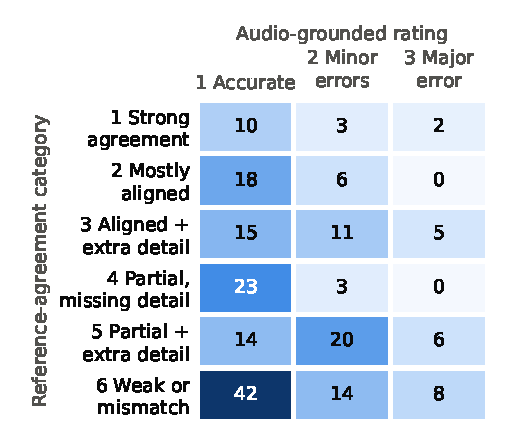
\includegraphics[width=\linewidth]{e17_e18_heatmap.pdf}
\caption{Reference-agreement category (rows, judged against the references only) by audio-grounded rating (columns,
judged against the recording) for the 200 sampled captions of all four models.}
\label{fig:heatmap}
\end{figure}

The sample was similar to the full set on the measured summary statistics (standardized differences of at most
0.37). Against the references, \af\ and \qwen\ agree most often with the main
content and \gem\ least often (Table~\ref{tab:review}). \gpt's most frequent deviation is omission: it has the most
captions in category~4.

Against the audio, the order changes. \gpt\ was rated accurate for 47 of 50 recordings (94\%, 95\% CI 84--98\%)
with no major error, while the other three models were rated accurate for 23 to 27 (46--54\%, intervals within
33--67\%) and had 5 to 9 major errors. The most direct evidence of missing reference content is phrase-level: of the
262 phrases that no reference supports, 64\% [58, 70] are audible in the recording, 28\% are not and 8\% cannot be
verified. Unsupported phrases occur in 26 of \gem's captions, 19 of \qwen's and 15 of \af's, but in only one of
\gpt's. At the caption level (Fig.~\ref{fig:heatmap}), only 8 of the 64 captions in category~6 have a major error,
and 23 of the 26 category-4 captions are rated accurate. Disagreement with the references is therefore mostly not
an acoustic error in this review; incomplete references are the likeliest explanation, although reference errors,
ambiguous sounds and reviewer judgement may contribute.

The metrics follow the reference review, not the audio review. Kendall's $\tau$ between each metric's model order and
the reference-review order is 0.67--1.00, but with the audio-review order it is 0--0.33 for every metric except CLAP
similarity (0.67). Mean scores fall from category~1 to category~6 on every metric (e.g. FENSE 0.68 to 0.28), but are
flat or reversed across audio ratings (rescaled BERTScore 0.29, 0.31 and 0.34 for ratings 1, 2 and 3). Within a
recording, across 156 caption pairs from 42 recordings with different audio ratings, concordance ranges from 0.39
(rescaled BERTScore) to 0.58 (MACE, 95\% CI [0.46, 0.69]; CLAP similarity 0.56 [0.45, 0.66]), and no metric differs
significantly from chance after Holm correction. The intervals are wide and compatible with both chance and useful
discrimination.

\section{Discussion}
\label{sec:discussion}

The results separate two properties that reference-based evaluation treats as one: agreement with the references and
correctness about the audio. The text metrics agree with each other, with the reference-only review and with the model
order of RQ1, but none of them showed evidence of following the audio review across models or within recordings. \gpt\ is the clearest
case: it ranks third or fourth on every text metric, yet its captions were rated most accurate, because its deviations
from the references are omissions and correct additional details rather than errors. The models' longer captions and
the negative length--score correlations suggest that part of the gap to the human baseline reflects the short,
generic style of Clotho's references rather than wrong content. We did not control for length, so this explanation
remains untested.

CLAP similarity, which compares the caption with the audio, is the only metric on which a model is not significantly
below the human baseline, and it comes closest to the audio-review order. For LALM captions we therefore
recommend reporting audio-aware metrics alongside reference-based ones and checking a sample of captions against the
audio before reading score differences as quality differences.

\section{Limitations}
\label{sec:limitations}

The audio ratings are single-reviewer judgements on 50 recordings, without an independent second listener; the
reviewer had read the references before listening, and the order of \af, \qwen\ and \gem\ in the audio review is not
stable (33\% of resamples). The concordance analysis has little power (156 pairs from 42 recordings), so the absence
of evidence that metrics track correctness is not evidence that they cannot. Each model was run with one prompt and
one decoding setting, and the training data of the API models are undisclosed, so overlap with Clotho cannot be ruled
out. Finally, the findings are limited to Clotho's everyday and environmental sounds. Future work should collect audio
ratings from several independent listeners who have not seen the references, report inter-rater agreement, and use a
larger sample to estimate concordance more precisely.

\section{Conclusion}
\label{sec:conclusion}

On Clotho v2.1, the open-weight LALMs agree most with the references (RQ1), but every model remains below a matched human baseline on every reference-based metric and
writes captions 1.4--1.9 times longer than humans (RQ2). Most captions that disagree with the references had no
major error against the audio, most details that no reference supports are audible, and the model ranked third or
fourth by every text metric was rated most accurate (RQ3). Reference agreement alone is therefore insufficient
evidence of acoustic correctness; claims about acoustic quality need evidence from the audio. Code and data:
\url{https://github.com/anandaswarup/lalm-acoustic-caption-eval}.

% Page 5 holds only the acknowledgments, the ethics statement and the references.
\clearpage

\section{Acknowledgments}
\label{sec:ack}

No funding was received for conducting this study. The authors have no relevant financial or nonfinancial interests
to disclose. We acknowledge Tampere University for the Clotho dataset.

\section{Compliance with Ethical Standards}
\label{sec:ethics}

This study uses the publicly available Clotho dataset and captions generated by AI models. No human participants were
recruited, and no ethical approval was required.

\bibliographystyle{IEEEbib}
\bibliography{refs}

\end{document}
